\chapter{Filters}
This chapter presents a variety of filters (low pass, high pass, band pass, and band reject) using either passive or active components. First and second order filters are presented so that an $n$th-order filter can be constructed by cascading these first and/or second order filters.
\par Some of these filters can be designed either as Butterworth or Chebyshev filters. Butterworth filters are characterized by their maximally flat magnitude in the pass band for all-pole filters (so that, for all-pole filters, they are the best approximation to an ideal filter in the pass band). Unfortunately, the magnitude of a Butterworth filter poorly approximates an ideal filter near the cutoff frequency in that the magnitude does not drop particularly sharply from the pass band to the stop band. Higher order Butterworth filters transition more sharply and thus better approximate an ideal filter, but they are still inferior to filters like the Chebyshev filter. Chebyshev filters' magnitude response best approximates an ideal filter for all-pole filters in that the magnitude drops very sharply from the pass band to the stop band, but their frequency response has ripples in the pass band (i.e. the magnitude oscillates in the pass band, particularly near the cutoff frequency). Higher order Chebyshev filters transition even more sharply than lower order Chebyshev filters. Thus, Butterworth and Chebyshev filters solve different problems -- the former approximates  an ideal filter best in the pass band while the latter is a better approximation near the cutoff frequency.\footnote{Johnson, David E., "Operational Amplifier Circuits: Design and Application", Prentice-Hall, 1982, pp. 107, 111}
% figure out where to put the tables for the coefficients

\section{Low pass filters}

\subsection{RC low pass passive filter}
\begin{center}
	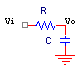
\includegraphics{schematics/rcLPfilter.PNG}
\end{center}
This is a very simple filter which can be easily analyzed using impedance. Viewing the resistor and capacitor as an impedance divider, $v_{o} = \frac{\frac{1}{sC}}{R+\frac{1}{sC}}v_{I}$. Rearranging, this is

\textcolor{red}{
\begin{equation}
\frac{v_{o}}{v_{i}}(s) = \frac{1}{sRC+1}
\label{eq:rcLPfilter}
\end{equation}
}

For low frequencies (s $\rightarrow$ 0) $\frac{v_{o}}{v_{i}} \approx 1$ (all the voltage falls across the capacitor) and for high frequencies (s $\rightarrow \infty$) $\frac{v_{o}}{v_{i}} \approx 0$ (the capacitor has very low impedance so $v_{O}$ is shorted to $GND$).

\subsection{First-order low pass active filter}
\begin{center}
	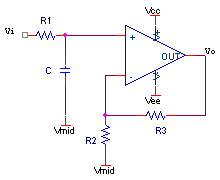
\includegraphics{schematics/1storderLPfilter.PNG}
\end{center}
The analysis of this circuit follows a similar approach as the op amp amplifier circuits. The voltage at the inverting input (and thus the non-inverting input) is $\frac{R_{2}}{R_{2}+R_{3}}v_{O}$ (assuming for simplicity that $v_{MID} = 0V$) since $R_{2}$ and $R_{3}$ form a voltage divider. KCL on the non-inverting input node then relates this voltage with the input. The transfer function is thus

\textcolor{red}{
\begin{equation}
\frac{v_{o}}{v_{i}}(s) = \frac{R_{2}+R_{3}}{R_{2}(sR_{1}C+1)}
\label{eq:1storderLPfilter}
\end{equation}
}

This is clearly a low pass filter since $\frac{v_{o}}{v_{i}} \approx 1+\frac{R_{3}}{R_{2}}$ for low frequencies where $sR_{1}C << 1$ (notice the circuit behaves like an op amp non-inverting amplifier here) and $\frac{v_{o}}{v_{i}} \approx 0$ for high frequencies where $sR_{1}C >> 1$. In the limiting cases where $R_{2} \rightarrow \infty$ and $R_{3} \rightarrow 0$ the op amp is configured like a voltage buffer with an RC low pass filter at its input -- $R_{2}$ and $R_{3}$ simply provide gain in addition to the filtering operation. If $R_{2}$ and $R_{3}$ are used, the three resistors should be chosen such that the filter formed by $R_{1}$ and $C$ has the desired -3dB frequency and $R_{1} = R_{2}||R_{3}$ (the latter relationship minimizes the error due to the op amp's input bias currents).
\par In this circuit $R_{1}$ and $C$ perform the same filtering function as the passive RC filter so the op amp isn't strictly necessary -- however, the op amp provides gain for the filter and can provide isolation of the RC filter from other circuit elements which might affect the its performance.

\subsection{Second-order VCVS low pass active filter}
\begin{center}
	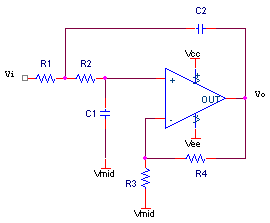
\includegraphics{schematics/2ndorder_vcvs_LPfilter.PNG}
\end{center}
This second order voltage controlled voltage source (VCVS) low pass filter is similar in topology to the the above first order low pass filter except that it includes an extra resistor and capacitor. The full derivation of the input/output relationship requires a somewhat lengthy manipulation of equations, but it requires only three facts: (1) the voltage at the input terminals, which is $\frac{R_{3}}{R_{3}+R_{4}}v_{o}$ (again assuming that $v_{MID} = 0V$), (2) the nodal equation at the non-inverting input, and (3) the nodal equation at the node common to $R_{1}$, $R_{2}$, and $C_{2}$. This circuit is a second order filter so the transfer function is of the form

\textcolor{red}{
\begin{equation}
\frac{v_{o}}{v_{i}}(s) = \frac{Kb\omega_{c}^{2}}{s^{2} + a\omega_{c}s + b\omega_{c}^{2}}
\label{eq:2ndorder_vcvs_LPfilter}
\end{equation}
}

In this case

\begin{equation}
b\omega_{c}^{2} = \frac{1}{R_{1}R_{2}C_{1}C_{2}}
\end{equation}
\begin{equation}
a\omega_{c} = \frac{1}{C_{2}}\left(\frac{1}{R_{1}} + \frac{1}{R_{2}}\right) - \frac{R_{4}}{R_{2}R_{3}C_{1}}
\end{equation}
\begin{equation}
K = 1 + \frac{R_{4}}{R_{3}}
\end{equation}

To minimize the error due to the op amp's input bias currents we need \begin{equation}
R_{3}||R_{4} = R_{1} + R_{2}
\end{equation}

With these restrictions and a desired gain K and -3dB angular frequency $\omega_{c}$ we have the following equations for deciding the resistor and capacitor values:\footnote{Ibid., pp. 118-119}
\begin{equation}
C_{1} \leq \frac{(a^{2}+4b(K-1))C_{2}}{4b}
\end{equation}
\begin{equation}
R_{1} = \frac{2}{(aC_{2}+\sqrt{(a^{2}+4b(K-1))C_{2}^{2} - 4bC_{1}C_{2}})\omega_{c}}
\end{equation}
\begin{equation}
R_{2} = \frac{1}{bC_{1}C_{2}R_{1}\omega_{c}^{2}}
\end{equation}
\begin{equation}
R_{3} = \frac{K(R_{1}+R_{2})}{K-1}, K > 1
\end{equation}
\begin{equation}
R_{4} = K(R_{1}+R_{2})
\end{equation}

The parameters $a$ and $b$ depend on the type of filter desired -- Butterworth or Chebyshev. See Appendix A for tables of these parameter values.
% add appendix for the Butterworth and Chebyshev a and b coefficient parameters

\subsection{Second-order biquad low pass filter}
\begin{center}
	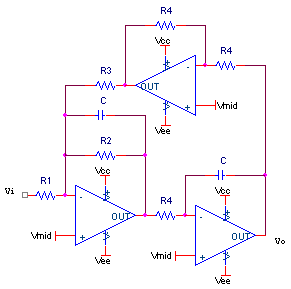
\includegraphics{schematics/2ndorderbiquadLPfilter.PNG}
\end{center}
The biquad filter requires two more op amps than the above VCVS filters. Two of the op amps are used as integrators and the third is an inverter. The two integrators (which, of course, are low pass filters) form a second order low pass filter. The transfer function can be determined by nodal analysis and noting the functions of each of the three op amps, but the full analysis is skipped. Instead, the resistors and capacitors are simply given in terms of the general second-order low pass filter transfer function

\textcolor{red}{
\begin{equation}
\frac{v_{o}}{v_{i}}(s) = \frac{Kb\omega_{c}^{2}}{s^{2} + a\omega_{c}s + b\omega_{c}^{2}}
\label{eq:2ndorderbiquadLPfilter}
\end{equation}
}

The resistors relate to the general transfer function as follows:
\begin{equation}
R_{4} = \frac{1}{\omega_{c}C}
\end{equation}
\begin{equation}
R_{1} = \frac{R_{4}}{Kb}
\end{equation}
\begin{equation}
R_{2} = \frac{R_{4}}{a}
\end{equation}
\begin{equation}
R_{3} = \frac{R_{4}}{b}
\end{equation}

Why use the biquad circuit with its three op amps when a second order filter can be built with only one op amp? Notice that the above equations for the biquad circuit's resistor and capacitor choices that the biquad is easier to tune than the VCVS filters. In particular, the desired $\omega_{c}$ determines the values of $C$ and $R_{4}$, and with $R_{4}$ chosen parameter $a$ is determined solely by $R_{2}$, parameter $b$ can be determined by $R_{3}$, and with $R_{3}$ determined $R_{1}$ can be used to set the filter's gain $K$. The VCVS filters require two different capacitor values and the resistors affect one or more values of $a$, $b$, and $K$ in nontrivial ways. The biquad circuit's offer of simpler tuning may be worth the two additional op amps.
\footnote{Ibid., pp. 120-122}

\section{High pass filters}

\subsection{RC high pass passive filter}
\begin{center}
	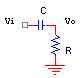
\includegraphics{schematics/rcHPfilter.PNG}
\end{center}
The resistor and capacitor have been switched in this case so the impedance divider is $v_{o} = \frac{R}{R+\frac{1}{sC}}v_{I}$. Rearranged, this is

\textcolor{red}{
\begin{equation}
\frac{v_{o}}{v_{i}}(s) = \frac{sRC}{sRC+1}
\label{eq:rcHPfilter}
\end{equation}
}

\subsection{First-order high pass active filter}
\begin{center}
	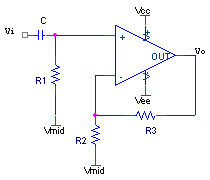
\includegraphics{schematics/1storderHPfilter.PNG}
\end{center}
Following the same approach as with the low pass active filter (using the resistor divider formed by $R_{2}$ and $R_{3}$ to calculate the op amp's input voltage in terms of $v_{o}$ and using KCL on the non-inverting input), the transfer function of the high pass filter is

\textcolor{red}{
\begin{equation}\frac{v_{o}}{v_{i}}(s) = \frac{sR_{1}C(1+\frac{R_{3}}{R_{2}})}{sR_{1}C+1}
\label{eq:1storderHPfilter}
\end{equation}
}

For low frequencies (s $\rightarrow$ 0) $\frac{v_{o}}{v_{i}} \approx 0$ and for high frequencies (s $\rightarrow \infty$) $\frac{v_{o}}{v_{i}} \approx 1 + \frac{R_{3}}{R_{2}}$ so the circuit behaves as a high pass filter. As usual, the resistors should be chosen such that $R_{1} = R_{2}||R_{3}$ to minimize the error due to the op amp's input bias currents. If gain is not needed, the op amp can be configured as a voltage buffer by removing $R_{2}$ and replacing $R_{3}$ with a short.

\subsection{Second-order VCVS high pass filter}
\begin{center}
	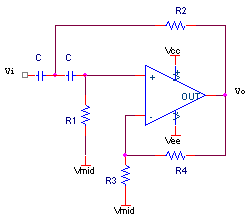
\includegraphics{schematics/2ndorder_vcvs_HPfilter.PNG}
\end{center}
The VCVS second-order high pass filter is the same as the VCVS second-order low pass filter but with the resistors replaced with capacitors and the capacitors replaced by resistors (except for the resister divider). Using the  general transfer function for a second-order high pass filter

\textcolor{red}{
\begin{equation}
\frac{v_{o}}{v_{i}}(s) = \frac{Ks^{2}}{s^{2} + \frac{a}{b}\omega_{c}s + \frac{\omega_{c}^{2}}{b}}
\label{eq:2ndorder_vcvs_HPfilter}
\end{equation}
}

the resistors determine the transfer function as follows:\footnote{Ibid., pp. 130-131}
\begin{equation}
R_{1} = \frac{4b}{(a+\sqrt{a^{2}+8b(K-1)})\omega_{c}C}
\end{equation}
\begin{equation}
R_{2} = \frac{b}{\omega_{c}^{2}C^{2}R_{1}}
\end{equation}
\begin{equation}
R_{3} = \frac{KR_{1}}{K-1}, K > 1
\end{equation}
\begin{equation}
R_{4} = KR_{1}
\end{equation}

If no gain is needed (i.e. $K = 1$) $R_{3}$ can be removed and $R_{4}$ replaced with a short.

\subsection{Second-order biquad high pass filter}
\begin{center}
	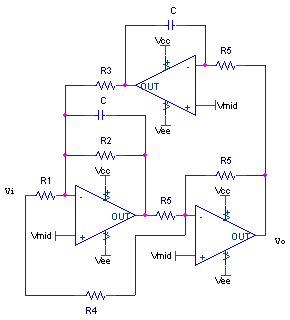
\includegraphics{schematics/2ndorderbiquadHPfilter.PNG}
\end{center}
This circuit is a biquad filter that implements the general second-order high pass filter transfer function

\textcolor{red}{
\begin{equation}
\frac{v_{o}}{v_{i}}(s) = \frac{Ks^{2}}{s^{2} + \frac{a}{b}\omega_{c}s + \frac{\omega_{c}^{2}}{b}}
\label{eq:2ndorderbiquadHPfilter}
\end{equation}
}

with an inverting gain (i.e. $K < 0$). The resistors relate to the transfer function as follows:\footnote{Ibid., p. 131}
\begin{equation}
R_{1} = \frac{b}{aK\omega_{c}C}
\end{equation}
\begin{equation}
R_{2} = KR_{1}
\end{equation}
\begin{equation}
R_{3} = \frac{b}{\omega_{c}C}
\end{equation}
\begin{equation}
R_{4} = \frac{1}{K\omega_{c}C}
\end{equation}
\begin{equation}
R_{5} = \frac{1}{\omega_{c}C}
\end{equation}

\section{Band pass filters}

\subsection{VCVS band pass filter}
\begin{center}
	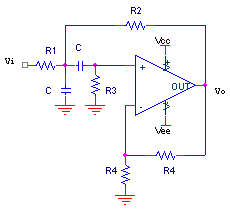
\includegraphics{schematics/vcvs_bandpass.PNG}
\end{center}
The general equation for the transfer function of this filter is

\textcolor{red}{
\begin{equation}
\frac{v_{o}}{v_{i}}(s) = \frac{\alpha \omega_{o}s}{s^{2}+\beta \omega_{o}s + \gamma \omega_{o}^{2}}
\label{eq:vcvs_bandpass}
\end{equation}
}

Since this is a band pass filter $\frac{v_{o}}{v_{i}} \approx 0$ as $s \rightarrow 0$ and $s \rightarrow \infty$ but the gain is nonzero in the midband. The resistors are related to the transfer function as follows:\footnote{Ibid., pp. 138-139}
\begin{equation}
R_{1} = \frac{2}{\alpha \omega_{o}C}
\end{equation}
\begin{equation}
R_{2} = \frac{2}{(-\beta+\sqrt{(\alpha - \beta)^{2} + 8\gamma})\omega_{o}C}
\end{equation}
\begin{equation}
R_{3} = \frac{1}{\gamma \omega_{o}^{2}C^{2}}\left(\frac{1}{R_{1}} + \frac{1}{R_{2}}\right)
\end{equation}
\begin{equation}
R_{4} = 2R_{3}
\end{equation}

\subsection{Biquad band pass filter}
\begin{center}
	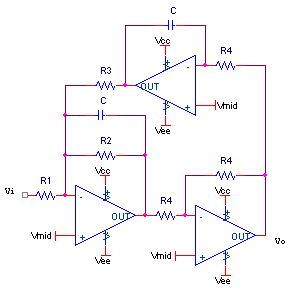
\includegraphics{schematics/biquad_bandpass.PNG}
\end{center}
The biquad band pass filter has the same transfer function as the VCVS band pass filter:

\textcolor{red}{
\begin{equation}
\frac{v_{o}}{v_{i}}(s) = \frac{\alpha \omega_{o}s}{s^{2}+\beta \omega_{o}s + \gamma \omega_{o}^{2}}
\label{eq:biquad_bandpass}
\end{equation}
}

with the four resistors related to the transfer function as
\begin{equation}
R_{1} = \frac{1}{\alpha \omega_{o}C}
\end{equation}
\begin{equation}
R_{2} = \frac{1}{\beta \omega_{o}C}
\end{equation}
\begin{equation}
R_{3} = \frac{1}{\gamma \omega_{o}C}
\end{equation}
\begin{equation}
R_{4} = \frac{1}{\omega_{o}C}
\end{equation}

Again, the VCVS band pass filter is simpler than the biquad but the latter is easier to tune than the former.\footnote{Ibid., p.140}

\section{Band reject filters}

\subsection{Passive Twin-T band reject filter}
\begin{center}
	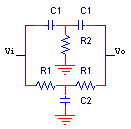
\includegraphics{schematics/passiveTwinTbandrejectfilter.PNG}
\end{center}
The intuitive way to understand that this circuit is a band reject filter is to realize that these are two T circuits in parallel -- one T circuit is composed of the two $R_{1}$ resistors and $C_{2}$ capacitor, and the other T circuit is composed of the two $C_{1}$ capacitors and $R_{2}$ resistor. Consider each T individually: the T circuit with the two resistors is a low pass filter since $C_{2}$ shorts the middle node to ground for high frequency signals and passes low frequency signals, and the T circuit with the two capacitors blocks low frequency signals but shorts $v_{i}$ to $v_{o}$ for high frequency signals. Low frequencies can pass through the low pass T circuit and high frequencies can pass through the high pass T circuit, but there is a middle frequency that can pass through neither. Thus, this Twin-T circuit is a band reject filter.
\par There are several methods for deriving the notch frequency $f = \frac{\omega}{2\pi}$ (the frequency which is attenuated the most), but the derivation is lengthy and not presented here. The result of the derivation is\footnote{Bond, C. \href{http://www.crbond.com/circuit\_analysis.htm}{http://www.crbond.com/circuit\_analysis.htm}}
\begin{equation}R_{1}C_{1} = 4R_{2}C_{2}
\end{equation}

and

\begin{equation}
\omega^{2} = \frac{1}{2R_{1}R_{2}C_{2}^{2}}
\end{equation}

Usually the components are chosen such that $R_{2} = \frac{R_{1}}{2}$ and $C_{2} = 2C_{1}$. In that case, the notch frequency is

\textcolor{red}{
\begin{equation}
f = \frac{\omega}{2\pi} = \frac{1}{2\pi R_{1}C_{1}}
\label{eq:passiveTwinTnotchfreq}
\end{equation}
}

The limitation of this circuit is its quality factor $Q = \frac{1}{\Delta\Omega}$, where $\Delta\Omega$ is the difference between the -3dB frequencies just above and below the notch frequency $f$. For the passive Twin-T band reject filter,

\textcolor{red}{
\begin{equation}
Q = \frac{1}{4}
\label{passiveTwinT_Q}
\end{equation}
}

An active Twin-T band reject filter (which uses the Twin-T topology in the feedback path of an operational amplifier) improves $Q$.\footnote{Mancini, Ron., "Op Amps for Everyone", Texas Instruments, Inc., 2002, p. 321}

\subsection{Passive Wien-Robinson band reject filter}
\begin{center}
	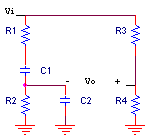
\includegraphics{schematics/passiveWien-Robinsonbandrejectfilter.PNG}
\end{center}
The Wien-Robinson band reject filter takes a single-ended input and produces a differential output. It can be analyzed intuitively by realizing that it is composed of a voltage divider ($R_{3}$ and $R_{4}$) in parallel with a band pass filter. $R_{1}$, $R_{2}$, $C_{1}$, and $C_{2}$ form a band pass filter because $C_{1}$ blocks low frequencies (no current passes through $C_{1}$ to create a voltage across $R_{2}$ and $C_{2}$) and $C_{2}$ shorts the band pass filter's output (the negative terminal of $v_{o}$) to ground, but midrange frequencies are passed to the output. The overall circuit acts as a band reject filter because at low and high frequencies the negative terminal of $v_{o}$ is grounded so that $v_{o} = \frac{R_{3}}{R_{2}+R_{3}}v_{i}$
At middle frequencies $v_{i}$ is passed to the negative terminal of $v_{o}$ so that the terminals of $v_{o}$ are equal and $v_{o} = 0$.
\par This circuit suffers from a low $Q$, just as the passive Twin-T band reject filter (the two have similar values of $Q$).\footnote{Mancini, Ron., "Op Amps for Everyone", Texas Instruments, Inc., 2002, p. 323} It too can be improved with the use of operational amplifiers.
\par Typically the component values are chosen such that $R_{1} = R_{2}$ and $C_{1} = C_{2}$. In that case the notch frequency is\footnote{Mancini, Ron., "Op Amps for Everyone", Texas Instruments, Inc., 2002, p. 324}

\textcolor{red}{
\begin{equation}
f = \frac{1}{2\pi R_{1}C_{1}}
\label{eq:passiveWienRobinson}
\end{equation}
}

\subsection{Active Twin-T band reject filter}
\begin{center}
	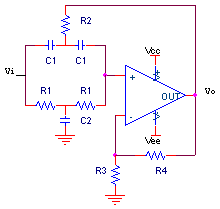
\includegraphics{schematics/activeTwinTbandrejectfilter.PNG}
\end{center}
The active Twin-T band reject filter adds an operational amplifer to the passive Twin-T filter. The operational amplifier provides an increased gain and $Q$ since it is an active element. $R_{4}$ provides negative feedback and $R_{3}$ sets the gain in the pass band (the filter circuitry has a gain of appoximately 1 in the pass band, so the circuit is essentially a non-inverting op amp amplifier). The pass band gain $K$ is thus simply

\textcolor{red}{
\begin{equation}
K = 1 + \frac{R_{4}}{R_{3}}
\end{equation}
}

The filter circuitry itself is configured the same as that of the passive Twin-T filter, with the passive version's output node connected to the operational amplifier's non-inverting input and $R_{2}$ connected to the active filter's output. Since the filter circuitry is the same, so is the notch frequency $f$. Assuming the typical case of $R_{2} = \frac{R_{1}}{2}$ and $C_{2} = 2C_{1}$,

\textcolor{red}{
\begin{equation}
f = \frac{1}{2\pi R_{1}C_{1}}
\end{equation}
}

It can be shown that the active Twin-T filter's $Q$ is\footnote{Mancini, Ron., "Op Amps for Everyone", Texas Instruments, Inc., 2002, p. 322}

\textcolor{red}{
\begin{equation}
Q = \frac{1}{2(2-k)} = \frac{R_{3}}{2(R_{3}-R_{4})}
\end{equation}
}

With $K$ and $Q$ given in terms of the circuit components, the overall transfer function can be written in terms of the circuit components as well:

\textcolor{red}{
\begin{equation}
\frac{v_{o}}{v_{i}}(s) = \frac{K(s^{2}+1)}{s^{2}+\frac{s}{Q}+1} =  \frac{\frac{R_{3}+R_{4}}{R_{3}}(s^{2}+1)}{s^{2}+\frac{2(R_{3}-R_{4})}{R_{3}}s+1}
\end{equation}
}

\subsection{Active Wien-Robinson band reject filter}
\begin{center}
	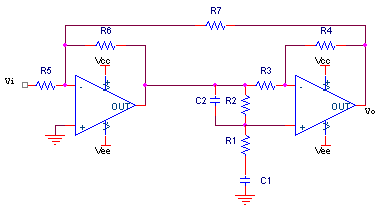
\includegraphics{schematics/activeWien-Robinsonbandrejectfilter.PNG}
\end{center}
The active Wien-Robinson band reject filter uses two operational amplifiers to improve the passive Wien-Robinson filter's $Q$ and gain. The resistors and capacitors which compose the passive Wien-Robinson filter are labeled the same in the above schematic of the active version as in the passive version from before. The inputs of the operational amplifier which drives the overall output are driven by the filter's differential output. The other operational amplifier is configured simply as an inverting amplifier. The transfer function can be written as\footnote{Mancini, Ron., "Op Amps for Everyone", Texas Instruments, Inc., 2002, p. 323}

\textcolor{red}{
\begin{equation}
\frac{v_{o}}{v_{i}}(s) = \frac{\frac{R_{6}R_{7}}{R_{5}(R_{6}+R_{7})}(s^{2}+1)}{s^{2}+\frac{3R_{7}}{R_{6}+R_{7}}s+1}
\label{eq:activeWienRobinsonbandreject}
\end{equation}
}

If $R_{1} = R_{2}$ and $C_{1} = C_{2}$ as is typical, then

\textcolor{red}{
\begin{equation}
f = \frac{1}{2\pi R_{1}C_{1}}
\end{equation}
}

since the filtering circuitry is unchanged from the passive version. $Q$ can be determined by inspection since it is the coefficient of the first order $s$ term,

\textcolor{red}{
\begin{equation}
Q = \frac{3R_{7}}{R_{6}+R_{7}}
\end{equation}
}

and the active filter's passband gain $K$ can also be determined by inspection:

\textcolor{red}{
\begin{equation}
K = \frac{R_{6}R_{7}}{R_{5}(R_{6}+R_{7})}
\end{equation}
}

The active Wien-Robinson band reject filter differs from its active Twin-T counterpart in that the passband gain $k$ can be chosen without affecting the quality factor $Q$.

\subsection{VCVS band reject filter}
\begin{center}
	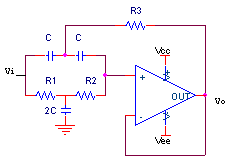
\includegraphics{schematics/vcvs_bandreject.PNG}
\end{center}
This band reject filter's transfer function can be written in the form

\textcolor{red}{
\begin{equation}
\frac{v_{o}}{v_{i}}(s) = \frac{s^{2} + \omega_{o}^{2}}{s^{2} + \frac{\omega_{o}}{Q}s + \omega_{o}^{2}}
\label{eq:vcvs_bandreject}
\end{equation}
}

The op amp is configured as a voltage follower and, since it is the only active device in the circuit, the overall gain of this filter can never exceed unity even in the pass band. To achieve the desired transfer function the resistors must be chosen as follows:\footnote{Ibid., pp. 145-146}
\begin{equation}
R_{1} = \frac{1}{2Q\omega_{o}C}
\end{equation}
\begin{equation}
R_{2} = \frac{2Q}{\omega_{o}C}
\end{equation}
\begin{equation}
R_{3} = \frac{R_{1}R_{2}}{R_{1}+R_{2}}
\end{equation}

\subsection{Biquad band reject filter}
\begin{center}
	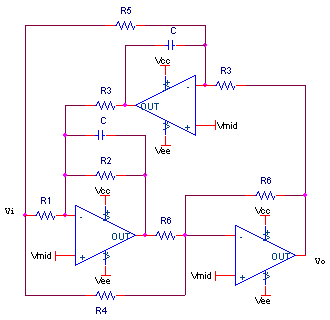
\includegraphics{schematics/biquad_bandreject.PNG}
\end{center}
A band reject filter's transfer function can also be written in the form 

\textcolor{red}{
\begin{equation}
\frac{v_{o}}{v_{i}}(s) = \frac{\alpha (s^{2} + \omega_{o}^{2})}{s^{2} + \beta \omega_{o}s + \gamma \omega_{o}^{2}}
\label{eq:biquad_bandreject}
\end{equation}
}

Unlike the VCVS band reject filter above, this biquad filter can provide an inverting gain greater than unity (the $\alpha$ term), and it can also achieve a much higher $Q$. The resistors relate to the transfer function as\footnote{Ibid., pp. 146-148}
\begin{equation}
R_{1} = \frac{1}{\alpha \beta \omega_{o}C}
\end{equation}
\begin{equation}
R_{2} = \alpha R_{1}
\end{equation}
\begin{equation}
R_{3} = \frac{1}{\sqrt{\gamma} \omega_{o}C}
\end{equation}
\begin{equation}
R_{4} = \frac{1}{\alpha \omega_{o}C}
\end{equation}
\begin{equation}
R_{5} = \frac{\sqrt{\gamma}}{\alpha \omega_{o}C}
\end{equation}
\begin{equation}
R_{6} = \frac{1}{\omega_{o}C}
\end{equation}

\section{All pass filters}
\subsection{First-order all pass filter}
\begin{center}
	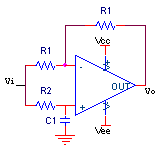
\includegraphics{schematics/1storderallpassfilter.PNG}
\end{center}
This circuit\footnote{Circuit courtesy of: Mancini, Ron., "Op Amps for Everyone", Texas Instruments, Inc., 2002, p. 328} has a gain of 1 at low frequencies and -1 at high frequencies. At low frequencies, neither the capacitor nor the non-inverting input of the operational amplifier draw any current, so there is no voltage drop across $R_{2}$ and the non-inverting input has a voltage equal to $v_{i}$. The inverting input also has a voltage equal to $v_{i}$ since the operational amplifier's inputs must be at (approximately) equal voltage, so there is no voltage drop across the $R_{1}$ connected to $v_{i}$. Since there is no voltage drop across (or current through) the $R_{1}$ connected to $v_{i}$, there is no current through (or voltage drop across) the $R_{1}$ connected to $v_{o}$. Thus, $v_{o} = v_{i}$ at low frequencies. At high frequencies, the non-inverting input of the operational amplifier is shorted to ground since the capacitor has a very low impedance. $R_{2}$ does nothing to the circuit since it is only connected to $v_{i}$ and $GND$ and the circuit looks like an inverting op amp amplifier, which of course has a gain of -1 when the gain and feedback resistors ($R_{1}$, in this case) are equal.
\par It is not intuitively obvious, however, that the circuit has a gain of magnitude 1 in the middle of the frequency spectrum, so we need to derive the transfer function. Let the voltage at the operational amplifier's inputs be $v_{x}$. $R_{2}$ and $C_{1}$ act as a voltage divider for $v_{i}$ at the operational amplifier's inverting input, so
\begin{equation}v_{x} = \frac{\frac{1}{sC_{1}}}{R_{2}+\frac{1}{sC_{1}}}v_{i} = \frac{v_{i}}{1+sR_{2}C_{1}}
\end{equation}
The operational amplifier's non-inverting input is also at voltage $v_{x}$ (ideally), so use KCL at the non-inverting input node:
\begin{equation}
\frac{v_{o}-v_{x}}{R_{1}} = \frac{v_{x}-v_{i}}{R_{1}}
\end{equation}
Substituting for $v_{x}$, we have \begin{equation}
\frac{v_{o}}{R_{1}}-\frac{v_{i}}{R_{1}(1+sR_{2}C_{1})} = \frac{v_{i}}{R_{1}(1+sR_{2}C_{1})}-\frac{v_{i}}{R_{1}}
\end{equation}
Rearranging, we have
\begin{equation}
v_{o} = v_{i}\left(\frac{2}{1+sR_{2}C_{1}}-1\right)
\end{equation}
Rearranging further, the transfer function is thus

\textcolor{red}{
\begin{equation}
\frac{v_{o}}{v_{i}}(s) = \frac{1-sR_{2}C_{1}}{1+sR_{2}C_{1}}
\label{eq:1storderallpassfilter}
\end{equation}
}

The transfer function reveals a zero at $s = \frac{1}{R_{2}C_{1}}$ and a pole at $s = -\frac{1}{R_{2}C_{1}}$ (technically, the operational amplifier introduces its own poles to the system so that the gain does actually go to zero at very high frequencies, but we are assuming that the frequencies of operation are well below the operational amplifier's poles). In any case, the gain has constant magnitude $|H(s)| = |H(j\omega)|$ across the (operational) frequency spectrum since

\begin{equation}
|H(j\omega)| = \frac{\sqrt{1+(-\omega R_{2}C_{1})^{2}}}{\sqrt{1+(\omega R_{2}C_{1})^{2}}} = 1
\end{equation}

so the circuit is an all pass filter. The point of an all pass filter is that it can change a system's phase response across the frequency spectrum -- the phase changes from $0$ to $-\pi$ radians from low to high frequency. More specifically, the phase $\angle H(s) = \angle H(j\omega)$ is

\textcolor{red}{
\begin{equation}
\angle H(j\omega) = \tan^{-1}(-\omega R_{2}C_{1}) - \tan^{-1}(\omega R_{2}C_{1}) = -2\tan^{-1}(\omega R_{2}C_{1})
\label{eq:1storderallpassfilter_angle}
\end{equation}
}

Although the values of $R_{2}$ and $C_{1}$ do not affect the magnitude of the circuit's gain across the frequency spectrum, they must be chosen appropriately to shape the circuit's phase response over frequency as desired. $R_{1}$ can be any reasonable value, of course, since the $R_{1}$ resistors do not directly affect the transfer function.

\subsection{Second-order all pass filter}
\begin{center}
	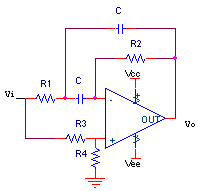
\includegraphics{schematics/2ndorder_allpass.PNG}
\end{center}
A second order all pass filter has the transfer function

\textcolor{red}{
\begin{equation}
\frac{v_{o}}{v_{i}}(s) = H(s) = \frac{K(s^{2} - a\omega_{o}s + b\omega_{o}^{2})}{s^{2} + a\omega_{o}s + b\omega_{o}^{2}}
\label{eq:2ndorder_allpass}
\end{equation}
}

since this transfer function has two poles and

\begin{equation}
|H(j\omega)| = K\frac{\sqrt{(b\omega_{o}^{2}-\omega^{2}) + (-a\omega_{o}\omega)^{2}}}{\sqrt{(b\omega_{o}^{2}-\omega^{2}) + (a\omega_{o}\omega)^{2}}} = K
\end{equation}

The phase $\angle H(j\omega)$ is

\textcolor{red}{
\begin{equation}
\angle H(j\omega) = \tan^{-1}\left(-\frac{b\omega_{o}^{2}-\omega^{2}}{a\omega_{o}\omega}\right) - \tan^{-1}\left(\frac{b\omega_{o}^{2}-\omega^{2}}{a\omega_{o}\omega}\right) = -2\tan^{-1}\left(\frac{b\omega_{o}^{2}-\omega^{2}}{a\omega_{o}\omega}\right)
\label{eq:2ndorder_allpass_angle}
\end{equation}
}

This circuit implements the second order all pass filter transfer function, with the resistors chosen such that
\begin{equation}
a\omega_{o} = \frac{2}{R_{2}C}
\end{equation}
\begin{equation}
b\omega_{o}^{2} = \frac{1}{R_{1}R_{2}C^{2}}
\end{equation}
\begin{equation}
K = \frac{R_{4}}{R_{3}+R_{4}}
\end{equation}
\begin{equation}
4R_{1}R_{4} = R_{2}R_{3}
\end{equation}
For minimum DC offset, choose\footnote{Ibid., pp. 151-153}
\begin{equation}
R_{2} = \frac{R_{3}R_{4}}{R_{3}+R_{4}}
\end{equation}